% -----------------------------------------------
% Resumo estendido no formato ISMIR (template oficial 2026)
% Compilar com pdfLaTeX + BibTeX (padrão do Overleaf)
% -----------------------------------------------
\documentclass{article}
\usepackage[T1]{fontenc}
\usepackage[utf8]{inputenc}
\usepackage[brazil]{babel}
\usepackage{ismir} % sem a opção "submission": versão com autores identificados
\usepackage{amsmath,amssymb,cite,url}
\usepackage{graphicx}
\usepackage{booktabs}
\usepackage{color}

\title{Corais à Maneira de Bach com Cadeias de Markov: \\ Ordem, Memorização e Harmonização Condicionada}

% ---- Preencha com seus dados ----
\oneauthor
  {Nome do Autor}
  {Instituição -- Programa / Disciplina\\\texttt{email@instituicao.br}}
\def\authorname{N. Autor}

\sloppy

\begin{document}
\maketitle

\begin{abstract}
Apresentamos um sistema de geração simbólica de ponta a ponta baseado exclusivamente em cadeias de Markov e restrito ao estilo dos corais a quatro vozes de J.\,S.~Bach. Uma cadeia de ordem~$n$, aprendida em 299 corais do \textit{music21}, gera a melodia do soprano como sequência de eventos (altura, duração, posição métrica, fermata). Uma cadeia de ordem~1 sobre sonoridades SATB a harmoniza por amostragem exata condicionada. Em varreduras de ordem, temperatura e suavização (30 peças por configuração), quantificamos o compromisso central do método: com $n\le2$ as frases perdem a regularidade do corpus, e com $n\ge5$ o modelo copia corais inteiros. A ordem $n=3$ equilibra estrutura e originalidade.
\end{abstract}

\section{Introdução}\label{sec:intro}
Cadeias de Markov estão entre as técnicas mais antigas de composição algorítmica~\cite{hiller1959,ames1989}: modelam o próximo evento dados os $n$ anteriores e, aprendidas de um corpus, reproduzem regularidades estilísticas locais sem codificar teoria musical. Implementamos com elas um sistema completo, do corpus ao MIDI e ao áudio.

\textbf{Restrição estilística.} A geração é restrita ao \emph{coral luterano a quatro vozes (SATB) no estilo de J.\,S.~Bach}: compasso 4/4, melodia em frases curtas delimitadas por fermatas, harmonização homofônica nota contra nota e cadência final sobre a tônica. É um banco de provas clássico em MIR~\cite{allan2005,hadjeres2017}.

\begin{figure*}[t]
\centering
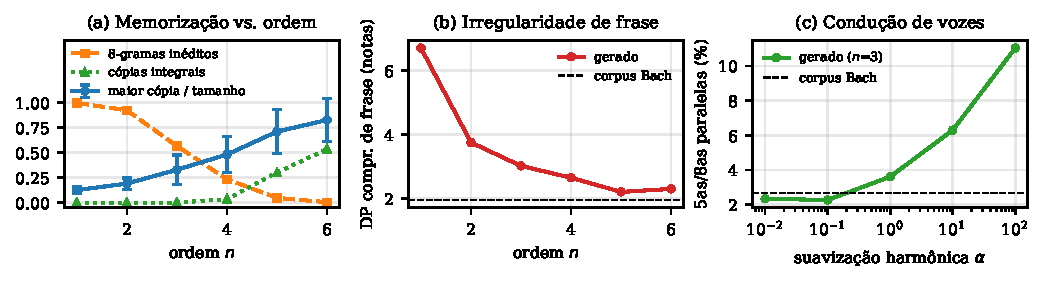
\includegraphics[width=\textwidth]{figures/sweeps.pdf}
\caption{Varreduras com 30 peças por configuração (modo maior). (a)~Memorização vs.\ ordem $n$: maior trecho idêntico a um coral (dividido pelo tamanho), 8-gramas (altura, duração) inéditos e fração de cópias integrais. (b)~Desvio-padrão do nº de notas por frase. (c)~Quintas/oitavas paralelas vs.\ suavização harmônica $\alpha$ ($n=3$).}
\label{fig:sweeps}
\end{figure*}

\section{Trabalhos Relacionados}\label{sec:related}
Cadeias de Markov aparecem já na \textit{Illiac Suite}~\cite{hiller1959}; Ames~\cite{ames1989} e Conklin~\cite{conklin2003} revisam modelos estatísticos em composição. O \textit{Continuator}~\cite{pachet2003} usa ordem variável para improvisar no estilo do intérprete, e Pachet e Roy~\cite{pachet2011} impõem restrições a sequências de Markov sem perder a distribuição aprendida, ideia usada em nossa harmonização. Papadopoulos et al.~\cite{papadopoulos2014} tratam explicitamente o plágio em ordens altas. Para corais de Bach, Allan e Williams~\cite{allan2005} harmonizam melodias com HMMs e DeepBach~\cite{hadjeres2017} usa redes neurais recorrentes.

\section{Método}\label{sec:method}
\textbf{Corpus e representação.} Dos 433 arquivos de Bach do \textit{music21}~\cite{cuthbert2010}, mantivemos corais em 4/4, a quatro vozes e sem melodias duplicadas: 299 peças (147 maiores, 152 menores; $\approx$7{,}5\,mil eventos por modo), transpostas para Dó maior ou Lá menor. Cada nota do soprano vira um evento $x_t=(p_t,d_t,b_t,f_t)$: altura MIDI, duração em semínimas, posição no compasso e \textit{flag} de fermata. $b_t$ garante coerência métrica e $f_t$ ensina onde terminam as frases (396 estados distintos no modo maior). Registra-se também a vertical $v_t=(p_t,a_t,t_t,b^{\text{baixo}}_t,f_t)$ soando no ataque de cada nota.

\textbf{Cadeia melódica de ordem $n$.} As probabilidades de transição são aprendidas do corpus por máxima verossimilhança,
\begin{equation}
P(x_t\mid x_{t-n}^{t-1}) = \frac{c(x_{t-n}^{t-1},x_t)}{c(x_{t-n}^{t-1})},
\end{equation}
com símbolos de início/fim, \textit{back-off} para ordens menores em contextos não vistos e temperatura $\tau$ ($p_i\propto c_i^{1/\tau}$). Por amostragem por rejeição, aceitam-se melodias com pelo menos 32 notas que terminem na tônica.

\textbf{Harmonização condicionada.} Uma cadeia de ordem~1 sobre verticais, suavizada por interpolação com a distribuição unigrama $P_0$,
\begin{equation}
P(v'\mid v)=\frac{c(v,v')+\alpha P_0(v')}{c(v)+\alpha},
\end{equation}
é amostrada \emph{condicionada} a que o soprano de cada $v_t$ coincida com a nota gerada e a que o baixo final seja a tônica. São restrições unárias~\cite{pachet2011}, satisfeitas por amostragem exata via \textit{forward-filtering/backward-sampling}~\cite{carter1994}, sem os becos sem saída de uma amostragem gulosa. A ordem~1 se deve à esparsidade: 1804 verticais distintas e só 4973 transições distintas observadas (modo maior).

\textbf{Escolha da ordem.} A esparsidade do corpus define o compromisso. O número de contextos distintos vai de 396 ($n=1$) a 5427 ($n=6$), e o número médio de sucessores por contexto cai de 12{,}5 para 1{,}8. A fração de ocorrências em contextos com um \emph{único} sucessor é de 3\%, 21\%, 49\%, 70\%, 81\% e 86\% para $n=1,\dots,6$. Com $n=1$ o modelo não sabe o tamanho de uma frase. Com $n\ge4$ ele percorre trechos inteiros do corpus sem alternativa. Adotamos $n=3$, em que metade das decisões ainda é aleatória.

\textbf{Saída.} Cada execução grava MIDI de quatro trilhas (\textit{pretty\_midi}~\cite{raffel2014}; órgão, 72\,bpm, fermatas prolongadas), MusicXML e JSON. O áudio é sintetizado com FluidSynth. A mesma semente reproduz a mesma peça.



\section{Resultados}\label{sec:results}
\textbf{Protocolo.} Geramos 30 peças (sementes fixas) por configuração em três varreduras: $n\in\{1,\dots,6\}$; $\tau\in\{0{,}5,\dots,3\}$ com $n=3$; e $\alpha\in\{10^{-2},\dots,10^{2}\}$ com $n=3$. Medimos \emph{memorização} (maior trecho idêntico a um coral; 8-gramas inéditos), \emph{fidelidade} (divergência de Jensen-Shannon de histogramas de altura, intervalo e duração; regularidade das frases), \emph{diversidade} (distância de edição entre peças) e \emph{condução de vozes} (quintas/oitavas paralelas).

\textbf{Resultados quantitativos.} Histogramas são reproduzidos por qualquer $n$ (JS de intervalos $<0{,}006$\,bits; $\approx$86\% de graus conjuntos, como em Bach) e não discriminam as configurações. O que muda com a ordem é a estrutura (Fig.~\ref{fig:sweeps}a,b): o desvio-padrão do comprimento de frase cai de 6{,}7 notas ($n=1$) para 2{,}2 ($n=5$), contra 1{,}9 no corpus, enquanto a fração copiada sobe de 12\% para 83\% e surgem cópias integrais a partir de $n=4$ (1, 9 e 16 das 30 peças com $n=4,5,6$). Com $n=3$, a peça típica reutiliza trechos de até cerca de 14 notas, mas 56\% dos seus 8-gramas não existem no corpus, e a diversidade entre peças (0{,}82) é próxima da observada entre corais reais (0{,}87). A temperatura tem efeito moderado ($n=3$): de $\tau=0{,}5$ a $2$, os 8-gramas inéditos vão de 52\% a 64\%, pois $\tau$ não altera contextos com escolha única. Já $\alpha$ controla diretamente a qualidade harmônica (Fig.~\ref{fig:sweeps}c): com $\alpha\le0{,}1$ a taxa de quintas/oitavas paralelas (2{,}3\%) é a mesma do próprio corpus (2{,}7\%) e sobe a 11\% com $\alpha=100$, quando a cadeia fica quase sem memória.

\begin{table}[t]
\centering\small
\setlength{\tabcolsep}{3pt}
\begin{tabular}{@{}lrrrlrrr@{}}
\toprule
Peça & $n$ & $\tau$ & $\alpha$ & Tom & notas & cópia máx. & paral. \\
\midrule
coral01 & 1 & 1{,}0 & 0{,}1 & Dó M & 44 & 7 & 2{,}3\% \\
coral02 & 3 & 1{,}0 & 0{,}1 & Dó M & 38 & 11 & 2{,}7\% \\
coral03 & 3 & 1{,}0 & 0{,}1 & Dó M & 38 & 13 & 5{,}4\% \\
coral04 & 2 & 1{,}5 & 0{,}1 & Ré m & 43 & 7 & 2{,}4\% \\
coral05 & 6 & 1{,}0 & 0{,}1 & Dó M & 49 & 49 (BWV 399) & 2{,}1\% \\
coral06 & 3 & 1{,}0 & 100 & Dó M & 38 & 11 & 5{,}4\% \\
\bottomrule
\end{tabular}
\caption{Peças de demonstração (áudio em \texttt{outputs/audio}). coral02 e coral03: mesma configuração, sementes diferentes.}
\label{tab:pieces}
\end{table}

\textbf{Análise qualitativa.} Áudios da Tabela~\ref{tab:pieces}: \url{https://github.com/SEU-USUARIO/bach-markov}. Em \textit{coral01} ($n=1$) as frases têm 6, 4, 24, 4 e 6 notas; uma vagueia por 24 notas até cadenciar no II grau: fragmentos plausíveis, sem arco formal. Em \textit{coral02} e \textit{coral03} ($n=3$) as frases têm de 5 a 9 notas (uma de 15), com cadências típicas: autênticas na tônica e semicadências na dominante, às vezes tonicizada (F$\sharp$). \textit{coral04} (Ré menor) termina com terça de picardia, traço idiomático de Bach. \textit{coral05} ($n=6$) é cópia integral do BWV~399. \textit{coral06} tem a melodia de \textit{coral02} e, com $\alpha=100$, o dobro de paralelas; por peça essa taxa é ruidosa (\textit{coral03}: 5{,}4\%), mas a tendência agregada (Fig.~\ref{fig:sweeps}c) é clara.

\section{Discussão e Trabalhos Futuros}\label{sec:discussion}
O sistema confirma o compromisso clássico: ordens baixas são fiéis localmente, mas sem forma; ordens altas atingem a regularidade de frase do corpus porque o reproduzem. Com $\approx$7{,}5\,mil eventos por modo, a janela útil é estreita ($n=3$).

Limitações: não há forma global (ex.: \textit{Barform} AAB); a tessitura pode derivar; as vozes internas só mudam nos ataques do soprano; regras de condução de vozes são aprendidas, não impostas. Propomos: modelos de ordem variável com restrição explícita de ordem máxima para impedir plágio~\cite{papadopoulos2014}; restrições de Markov para impor forma e tessitura~\cite{pachet2011}; harmonização com mais contexto (ex.: HMM sobre graus harmônicos~\cite{allan2005}); e um teste de audição com participantes para substituir a avaliação qualitativa aqui feita pelo próprio autor.

\bibliography{refs}

\end{document}
